\documentclass[11pt,oneside]{report}

% PACKAGES
\usepackage{graphicx}
\usepackage[labelfont=bf]{caption}
\usepackage{subcaption}
\usepackage[a4paper,width=160mm,top=20mm,bottom=20mm]{geometry}
\usepackage{fancyhdr}
\usepackage{hyperref}
\usepackage{overpic}
\usepackage{amsmath}
\usepackage{amsfonts}
\usepackage[acronym]{glossaries}
\usepackage{lipsum} %DUMMY TEXT
\usepackage{microtype}
\usepackage[utf8]{inputenc}
\usepackage{titlesec}
\usepackage{float}
\usepackage[style=nature, backend=biber]{biblatex}

% CONFIGS
\pagestyle{fancy}
\setlength{\headheight}{14.49998pt}
\fancyhead{}
\fancyhead[RO,LE]{Heavy-Tailed Initialisation as a New Paradigm in Continual Learning}
\fancyfoot{}
\fancyfoot[LO,CE]{\ifnum\value{chapter}=0\else \leftmark \fi}
\fancyfoot[LE,RO]{\thepage}
\hypersetup{
    pdfauthor = {Yi Hao},
    pdftitle = {Heavy-Tailed Initialisation as a New Paradigm in Continual Learning},
    colorlinks,
    linkcolor={blue},
    citecolor={blue},
    linkcolor={blue},
    citecolor={blue}
}
\PassOptionsToPackage{unicode}{hyperref}

% MACROS
% essentials
\renewcommand{\headrulewidth}{0.4pt}
\renewcommand{\footrulewidth}{0.4pt}
% non-essentials (some examples)
\newcommand{\unit}[1]{\ensuremath{\, \mathrm{#1}}}  % makes writing units simpler
\renewcommand{\thefootnote}{\emph{\alph{footnote}}} % italic letters footnote

% PATHS
\graphicspath{ {imgs/} }

% BIB SETUP
\addbibresource{references.bib}

% TITLE FORMATING
% Change [display] to [block] to put everything on one line
\titleformat{\chapter}[block]
{\normalfont\huge\bfseries} % Style of the entire line
{\chaptertitlename\ \thechapter:\quad} % Label (e.g., Chapter 1:)
{0pt} % Space between label and title (0pt because \quad handles it)
{\huge} % Style for the title text

% Adjust the spacing to move it up
\titlespacing*{\chapter}{0pt}{-10pt}{20pt}


% <><><><><><><><><><><><><><><><><><><><><><>
\begin{document}

% ---------------------------------------------------------
% PAGE 1: TITLE PAGE
% ---------------------------------------------------------
\pagenumbering{arabic} % Start numbering here
\begin{titlepage}
	\addcontentsline{toc}{chapter}{Title Page} % Add to TOC
    \begin{center}
        \vspace*{1cm}
        
        \Huge
        \textbf{Heavy-Tailed Initialisation as a New Paradigm in Continual Learning}
        
        \vspace{1.5cm}
        
        \Large{Yi Hao}
        
        \vfill
        
        \large
        A thesis presented for the degree of\\
        Bachelor of Science (Honours) (Physics)
        
        \vspace{0.8cm}
        
        
\includegraphics[width=0.4\textwidth]{usyd_logo.png}
        
        \large
        School of Physics\\
        Faculty of Science\\
        The University of Sydney\\
        Australia\\
        \today

        \vfill

        {\Large Supervisor: Prof.\;Pulin Gong}
        
        \vspace{1cm}
        \large{1} % Manually placing the page number 1 at the bottom
    \end{center}
\end{titlepage}
\setcounter{page}{2}

% ---------------------------------------------------------
% PAGE 2: ABSTRACT
% ---------------------------------------------------------
\clearpage
\addcontentsline{toc}{chapter}{Abstract} % Add to TOC before the chapter starts
\chapter*{Abstract}
\lipsum[1-2]

% ---------------------------------------------------------
% PAGE 3: STATEMENTS & ACKNOWLEDGEMENTS
% ---------------------------------------------------------
\clearpage
% Anchor both to Page 3 in the TOC
\addcontentsline{toc}{chapter}{Statement of Originality}
\addcontentsline{toc}{chapter}{Acknowledgements}
\addcontentsline{toc}{chapter}{Statement of Contribution}

\chapter*{Statements and Acknowledgements}

\section*{Statement of Originality}
I certify that this thesis contains work carried out by myself except where otherwise acknowledged.
\vspace{0.5cm}
\noindent Signed: \rule{4cm}{0.4pt} \hfill Date: \today

\section*{Acknowledgements}
\lipsum[3]

\section*{Statement of Contribution}
\lipsum[4-5]

% ---------------------------------------------------------
% PAGE 4: TABLE OF CONTENTS
% ---------------------------------------------------------
% Rule: If this takes >1 page, only the first counts toward the 40 limit.
\clearpage
\addcontentsline{toc}{chapter}{Contents}
\tableofcontents
\clearpage

% ---------------------------------------------------------
% MAIN CONTENT (Page 5+)
% ---------------------------------------------------------

\addcontentsline{toc}{chapter}{Introduction}
\chapter*{Introduction}
\label{chap:intro}
Deep neural networks have achieved widespread success across modern domains, from language models to medical diagnostics and autonomous robotics. However, standard training relies on fixed, independent, and identically distributed (i.i.d.) datasets. Truly intelligent systems must instead possess the capacity for continual learning, acquiring knowledge over time from evolving data streams without retraining from scratch. This capability is essential for dynamic real-world environments and serves as a key step toward mimicking biological intelligence. Yet, transitioning neural networks from static to continual learning reveals a major vulnerability: when adapted to new tasks, models systematically overwrite prior knowledge, encountering the stability-plasticity dilemma.

The stability-plasticity dilemma reflects a trade-off in how neural networks encode and retain information. To learn a new task, a network requires plasticity to update its parameters and integrate new information. Conversely, retaining past information demands stability to preserve configurations established during prior training. In standard optimisation, parameter updates driven by a new task alter the space dedicated to earlier tasks, causing a sudden collapse in past performance known as catastrophic forgetting. Because standard architectures treat parameters as a shared medium, improving plasticity almost invariably degrades stability, forcing a trade-off between learning capacity and memory retention. To navigate this, researchers have devised various strategies to preserve memory.

While these algorithmic interventions have yielded significant progress, they share a common design choice: they act strictly after initialisation. Across these diverse approaches, the initial state of the network is treated as a passive choice, relying on standard Gaussian schemes to stabilise training at step zero. However, this reliance assumes that Gaussian weight distributions are the optimal starting point for continual learning, an assumption that remains largely unexamined. By treating initialisation as a fixed starting point rather than a structural variable, existing methods patch knowledge loss without testing whether initial weight geometry itself drives catastrophic forgetting. This gap motivates an alternative approach: configuring the initial weight geometry directly using non-Gaussian distributions.

A rigorous physical foundation for this paradigm shift stems from non-Gaussian statistical mechanics and random matrix theory. Replacing standard Gaussian assumptions with a generalised non-Gaussian framework, our research group has demonstrated that heavy-tailed initialisation induces an extended critical regime. Unlike conventional architectures that require delicate fine-tuning along a narrow edge of chaos, heavy-tailed networks establish a broad parameter region where learning signals propagate robustly without fine-tuning. Within this regime, the system's local dynamical operators exhibit spatially multifractal modes, combining localised activity with delocalised backgrounds in a manner analogous to Anderson transitions in disordered physical media.  

For deep learning systems, this network geometry provides two functional advantages: it exhibits directional symmetry breaking, expanding useful signal directions while contracting noise, and gives rise to a broad spectrum of intrinsic relaxation timescales. Consequently, heavy-tailed initialisation transforms the initial weight space from a passive background into an active physical state pre-conditioned to sustain robust representations over extended periods of learning. This theoretical framework suggests that networks can be initialised directly into a self-regularised phase space, closely mirroring the structural properties that high performing models typically achieve only after extensive optimisation. 

This picture is directly supported by empirical observations of neural network training dynamics. Frameworks such as heavy-tailed self-regularisation demonstrate that as deep neural networks learn, their weight spectra universally evolve away from random-matrix bulk distributions towards a power-law decay. Similarly, the training process exhibits heavy-tailed characteristics that allow optimisers to traverse high-dimensional loss landscapes via discrete jump processes rather than standard Brownian motion. These findings suggest that heavy-tailed geometry represents the natural end-state of well-trained models. Initiating training from standard Gaussian distributions therefore forces networks to waste optimisation capacity constructing this non-Gaussian structure from scratch.  

In this thesis, we evaluate heavy-tailed initialisation as a fundamental structural approach to addressing the longstanding challenges of continual learning. We focus specifically on Gradient Projection Memory (GPM), a subspace-constrained method that preserves past knowledge by projecting gradient updates orthogonally to past feature representations. GPM provides a clean, deterministic framework for our evaluation because it operates directly on intermediate representation geometry and offers explicit metrics to track capacity usage. By restricting parameter updates to orthogonal projections within a fixed-capacity network, GPM isolates how the weight geometry allocates space without introducing extra heuristics. However, standard GPM suffers from subspace saturation, where high-rank activations rapidly fill the available representation volume and cause a premature loss of plasticity. Our results demonstrate that applying heavy-tailed initialisations creates an extended critical regime that persists across sequential task environments. By inducing directional symmetry breaking and compressing feature rank, heavy-tailed initialisations allow the network to sustain higher average task accuracy and preserve long-term plasticity across a broad parameter range while occupying significantly less subspace capacity than conventional Gaussian initialisations.  

In Chapter 1, we review the foundational literature across continual learning, non-Gaussian statistical mechanics, and Gradient Projection Memory (GPM), establishing the theoretical mechanisms of extended criticality and identifying subspace saturation as the primary capacity bottleneck. In Chapter 2, we investigate the geometric properties of intermediate representations, analysing how heavy-tailed initialisation induces directional symmetry breaking to compress spectral rank and reduce basis consumption across fully connected and convolutional benchmarks. In Chapter 3, we examine the resulting continual learning dynamics, demonstrating why the preservation of residual gradient volume directly translates to superior task retention and long-term plasticity across sequential task horizons. In Chapter 4, we evaluate architectural scaling, testing the persistence of the extended critical regime and rank compression in modern deep topologies such as ResNet architectures. Finally, in Chapter 5, we synthesise our empirical findings within our broader statistical physics framework, discuss implications for deep learning theory, and outline directions for future research.

\chapter{Literature Review}
\label{chap:review}

In this thesis, we investigate heavy-tailed initialisation as a structural approach to catastrophic forgetting and loss of plasticity in continual learning. Because this work bridges non-Gaussian statistical mechanics, random matrix theory, and continual learning, fields that have largely developed independently, this chapter establishes the theoretical foundations underpinning our study. In Section 1.1, we outline the mathematical foundations of deep networks, formalise the stability-plasticity dilemma, and define standard continual learning evaluation scenarios. In Section 1.2, we review heavy-tailed network theory, covering Lévy mean-field theory, extended criticality, and multifractal representation geometry. Finally, in Section 1.3, we examine Gradient Projection Memory (GPM), detailing its subspace projection mechanics and identifying subspace saturation as its primary bottleneck.

\section{Continual Learning}
\subsection{Basics of Deep Neural Networks}
At its core, a deep neural network is a non-linear function approximator designed to discover meaningful mappings between an input space and an output space. Given a dataset of labelled training pairs $\mathcal{D} = \{(\mathbf{x}_i, \mathbf{y}_i)\}_{i=1}^N$, where $\mathbf{x}_i$ represents an input measurement and $\mathbf{y}_i$ is its corresponding correct output, the network parameterises this global relationship as a function $F(\mathbf{x}; \mathbf{w})$. Here, $\mathbf{w}$ represents the collective set of all trainable parameters distributed across the architecture.

Rather than attempting to map raw inputs directly to final targets in a single step, deep networks achieve high expressive power by passing information through a sequence of intermediate processing stages, known as hidden layers. As illustrated in Figure~\ref{fig:mlp_schematic}, for a network composed of $L$ layers, signal propagation begins by setting the initial state to the input, $\mathbf{x}^0 = \mathbf{x}$. At each subsequent layer $l \in \{1, \dots, L\}$, the internal state is computed through a two-step transformation:
\begin{equation}
	\mathbf{h}^l = \mathbf{W}^l \mathbf{x}^{l-1} + \mathbf{b}^l, \quad \mathbf{x}^l = \phi(\mathbf{h}^l)
\end{equation}
First, the incoming signal $\mathbf{x}^{l-1}$ undergoes a transformation parameterised by a weight matrix $\mathbf{W}^l \in \mathbb{R}^{d_l \times d_{l-1}}$ and a bias vector $\mathbf{b}^l \in \mathbb{R}^{d_l}$, yielding the pre-activation state $\mathbf{h}^l$. Second, this state is passed through an element-wise, non-linear activation function $\phi(\cdot)$, such as a hyperbolic tangent ($\tanh$) or rectified linear unit ($\mathrm{ReLU}$), to produce the post-activation representation $\mathbf{x}^l$. 

The inclusion of non-linear activations is essential: without them, an arbitrarily deep network collapses into a succession of linear matrix multiplications, offering no greater representational capacity than a single-layer model. By interleaving linear projections with non-linear functions, the network untangles complex data manifolds, isolating task-relevant features as the signal moves toward the final output layer $\hat{\mathbf{y}} = \mathbf{x}^L$.

\begin{figure}[htbp]
	\centering
	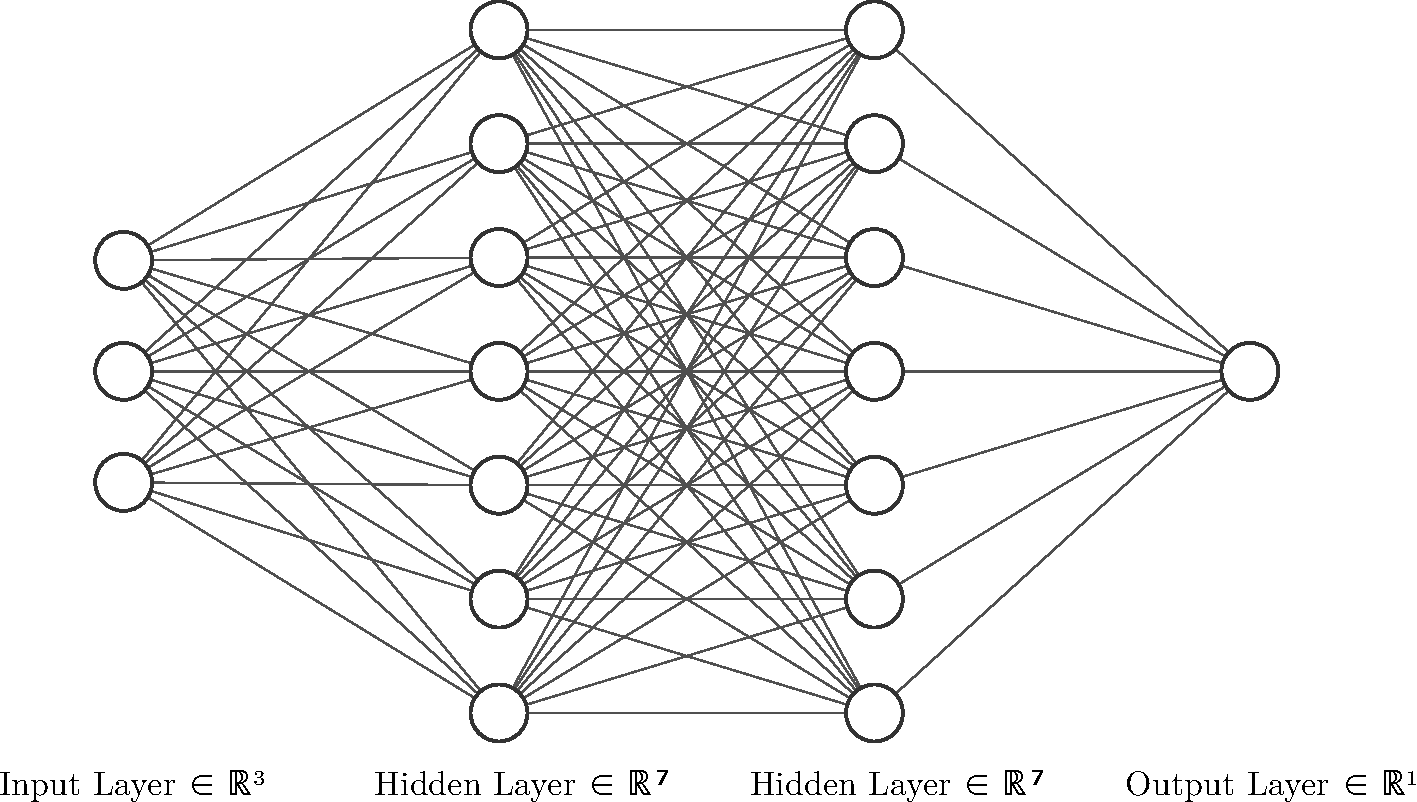
\includegraphics[width=0.7\textwidth]{imgs/nn_diagram.pdf}
	\vspace*{-0.5em}
	\caption{\textbf{Architecture of a fully connected feedforward neural network.} Signals propagate sequentially from input $\mathbf{x}^0 \in \mathbb{R}^3$ through intermediate hidden representations in $\mathbb{R}^7$ via weight transformations $\mathbf{W}^l$ and non-linearities $\phi(\cdot)$ to generate predictions $\hat{\mathbf{y}} \in \mathbb{R}^1$.}
	\label{fig:mlp_schematic}
	\vspace*{-0.5em}
\end{figure}

To evaluate how accurately the network approximates the true data distribution, its predictions $\hat{\mathbf{y}}_i = F(\mathbf{x}_i; \mathbf{w})$ are measured against the ground-truth targets $\mathbf{y}_i$ through a loss function $L(\mathbf{w})$:
\begin{equation}
	L(\mathbf{w}) = \frac{1}{N} \sum_{i=1}^N \mathcal{L}\left(F(\mathbf{x}_i; \mathbf{w}), \mathbf{y}_i\right)
\end{equation}
where $\mathcal{L}$ is a measure of distance between the prediction $\hat{\mathbf{y}}_i$ and the true value $\mathbf{y}_i$, such as mean squared error for continuous regression problems or cross-entropy for discrete classification. 

From a geometric and physical perspective, the loss $L(\mathbf{w})$ defines a loss landscape over the high-dimensional parameter space $\mathbb{R}^D$. The fundamental goal of training is to navigate this landscape to locate a minimising configuration $\mathbf{w}^* = \arg\min_{\mathbf{w}} L(\mathbf{w})$ that yields low prediction error on seen training samples while generalising well to unseen test data. 

Because non-linear activation functions render this objective landscape highly non-convex, finding $\mathbf{w}^*$ analytically is intractable. Instead, optimisation relies on gradient-based iterative search. In standard gradient descent, the parameter vector moves continuously down the local gradient of the loss surface:
\begin{equation}
	\mathbf{w}_{t+1} = \mathbf{w}_t - \eta \nabla L(\mathbf{w}_t)
\end{equation}
where $\mathbf{w}_t$ denotes the parameter state at step $t$, $\nabla L$ is the gradient vector pointing in the direction of steepest loss ascent, and $\eta > 0$ is the learning rate governing step size.

In real-world applications with massive datasets, evaluating the exact gradient $\nabla L$ over all $N$ data points at every iteration is computationally infeasible. Practical deep learning systems therefore utilise Stochastic Gradient Descent (SGD), which approximates the global gradient using a small, randomly sampled mini-batch $\mathcal{B} \subset \mathcal{D}$ of size $B \ll N$:
\begin{equation}
	\mathbf{w}_{t+1} = \mathbf{w}_t - \eta \nabla L_{\mathcal{B}}(\mathbf{w}_t)
\end{equation}
The mini-batch approximation introduces stochastic fluctuations into the optimisation trajectory. Rather than behaving as pure numerical noise, they act similarly to thermal fluctuations in a physical system. They help the optimiser overcome shallow barriers, and escape saddle points alongside local minima, guiding the parameter configuration into robust regions that offer superior generalisation.
\subsection{Continual Learning and the Stability-Plasticity Dilemma}
While standard deep learning assumes that training data is static alongside being independent and identically distributed (i.i.d.), real-world intelligent systems must operate in dynamic, non-stationary environments. Continual learning formalises this setting as a sequential process where a network learns across a continuous stream of distinct tasks $\mathcal{D}_1, \mathcal{D}_2, \dots, \mathcal{D}_T$. At any point in the sequence, the model must adapt its parameters to the current task distribution $\mathcal{D}_t$ under the constraint that data from previous tasks $\mathcal{D}_{<t}$ is either severely restricted or entirely inaccessible.

When standard deep neural networks adapt to shifting data distributions without constraints, they become exposed to two distinct failure modes. The first is catastrophic forgetting: when training on a new task using standard SGD, parameter updates move strictly along the gradient of the current loss surface. As illustrated in Figure~\ref{fig:continual_learning}, unconstrained gradient steps $g$ displace the parameter configuration out of the low-loss regions established for earlier tasks, overwriting previous feature mappings and causing past task performance to collapse abruptly. Conversely, prolonged sequential training over extended task sequences can trigger the opposing failure mode: the loss of plasticity. Rather than forgetting the past, the network progressively loses its capacity to learn in the future. Repeated parameter updates can push neurons into the flat, saturated regions of activation functions like $\tanh$, causing local gradients to vanish. At the same time, internal representations can collapse into narrow, redundant subspaces. This leaves the network functionally rigid and unable to adapt to new tasks.  

\begin{figure}[htbp]
	\centering
	\vspace*{-3em}
	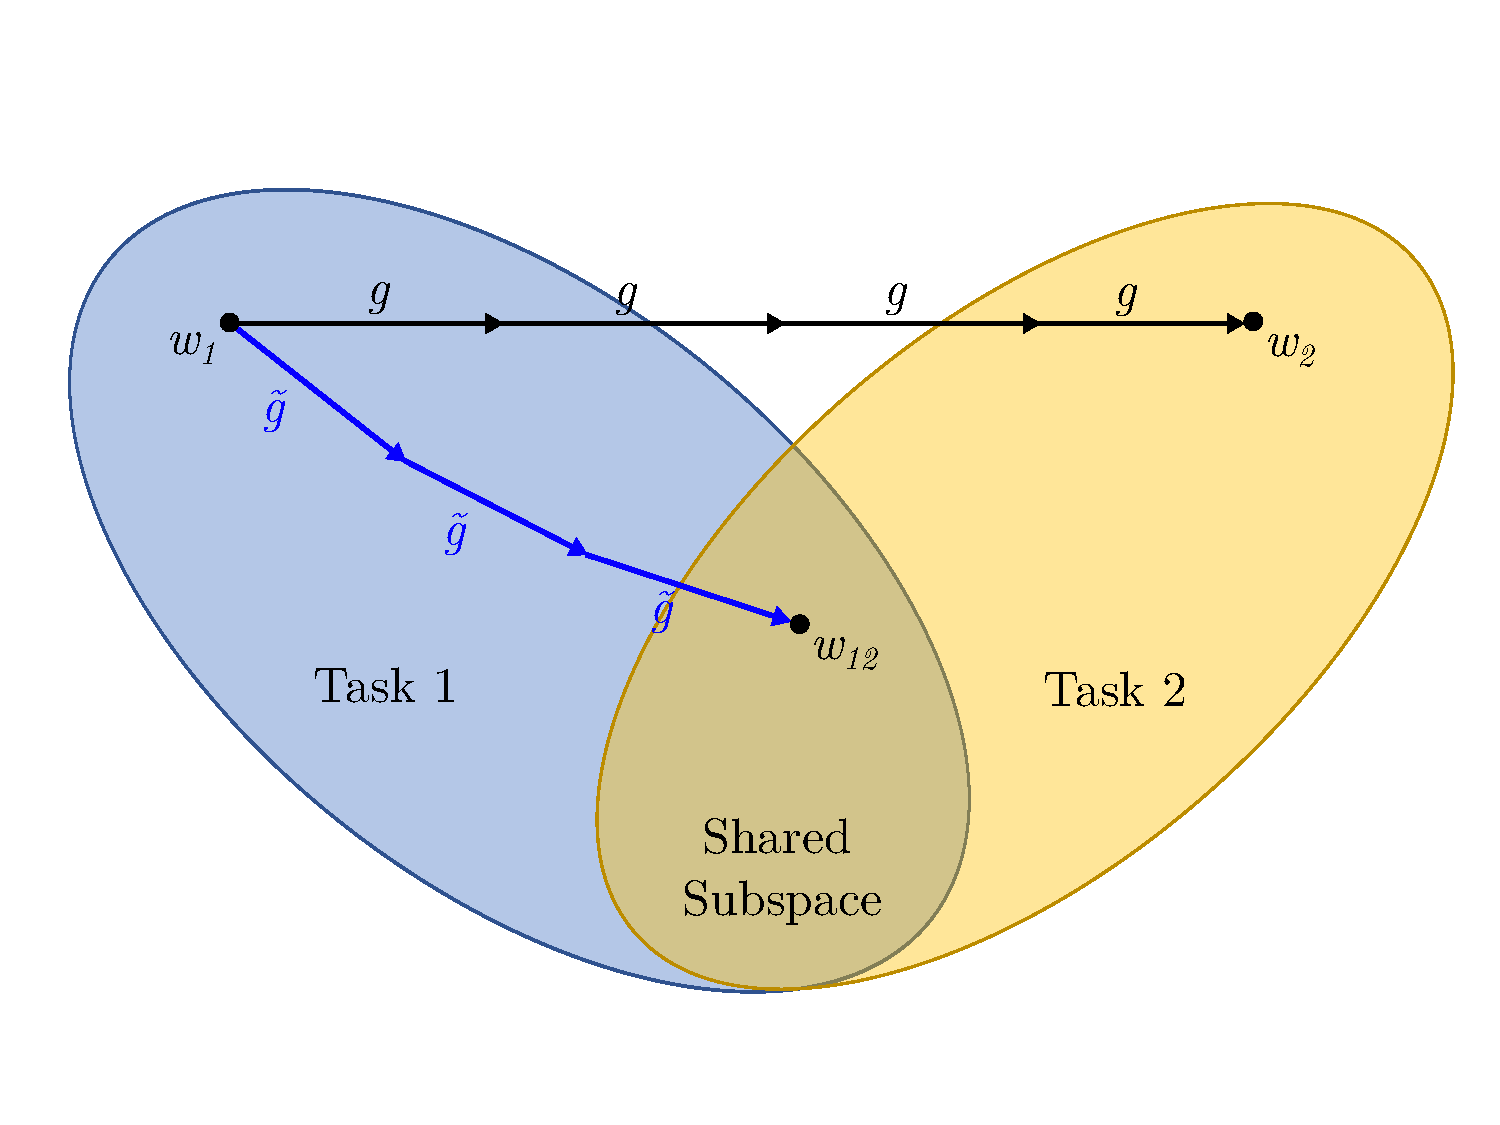
\includegraphics[width=0.7\textwidth]{imgs/continual_learning.pdf}
	\vspace*{-2em}
	\caption{\textbf{Geometric trajectories of standard versus continual learning across sequential tasks.} Starting from a converged configuration $w_1$ on Task 1, normal optimisation updates $g$ (black path) adapt purely to Task 2, driving parameters toward $w_2$ and leaving the Task 1 subspace, which results in catastrophic forgetting. In contrast, continual learning algorithms constrain updates $\tilde{g}$ (blue path) to remain compatible with past representations, guiding the parameter trajectory into a joint configuration $w_{12}$ within the shared subspace to retain past knowledge while learning the new task.}
	\label{fig:continual_learning}
\end{figure}

These complementary failure modes reflect a tension known as the stability-plasticity dilemma. Plasticity is the network's capacity to alter its parameters and integrate new information, whereas stability is the ability to preserve established configurations and protect past knowledge. Because standard deep architectures share a single parameter space across all tasks, optimising for immediate performance destabilises past configurations, while excessively freezing parameters eliminates future learning. Consequently, an effective continual learning system has to satisfy a dual mandate: enforcing structural stability to prevent catastrophic forgetting while preserving parameter flexibility and representation diversity to maintain long-term plasticity.
\subsection{Evaluation Scenarios in Continual Learning}
To systematically evaluate how algorithms navigate the stability-plasticity dilemma, continual learning benchmarks are categorised by whether task identity is accessible during inference. As formalised by van de Ven and Tolias (2019, 2022), these environments fall into three distinct scenarios: task-incremental, domain-incremental, and class-incremental learning. 

In task-incremental learning, task identity is explicitly provided at test time, allowing the network to route inputs through task-specific networks and isolating the primary challenge to preserving internal feature representations. Domain-incremental learning hides task identity during inference while maintaining a fixed output space, requiring the model to handle sequential shifts in the input data distribution. Class-incremental learning presents the most challenging scenario: task identity remains hidden, and the output space expands dynamically as novel classes arrive, requiring the network to discriminate across all learned classes simultaneously without suffering from output bias or representational collapse.

Evaluating fixed-capacity networks across these non-stationary environments typically requires structural constraints to preserve historical representations without storing past data buffers. While conventional methods apply algorithmic interventions strictly post-initialisation, their performance remains bounded by how internal representations occupy space within the network. Existing approaches rely largely on standard Gaussian schemes, treating initialisation as a passive step rather than an active physical determinant of representation geometry. In Section 1.2, we examine non-Gaussian statistical mechanics and random matrix theory, establishing how heavy-tailed initialisations induce extended criticality and compact, low-rank representation structures to support sequential learning.
\section{Heavy-Tailed Theory and Extended Criticality}
A neural network's dynamical capabilities are fundamentally governed by its initial parameter distribution. While classical theories assume Gaussian weights, confining stable signal propagation to a fragile, fine-tuned edge of chaos, empirical networks universally evolve heavy-tailed weight and singular value spectra. Grounded in non-Gaussian statistical physics and random matrix theory, heavy-tailed initialisation establishes an extended critical regime at step zero that sustains deep signal propagation, balances feature compression with expansion, and induces compact, low-dimensional representation geometries across parameter space.

\subsection{Heavy-Tailed Coupling and L{\'e}vy Mean-Field Theory}
To construct a physical description of networks with heavy-tailed connectivity, microscopic weights and biases are modelled using symmetric L{\'e}vy $\alpha$-stable distributions. A random variable $X \sim S_\alpha(\sigma)$ is parameterised by a characteristic tail index $\alpha \in [1, 2]$ and a scale parameter $\sigma > 0$. While $\alpha = 2$ recovers a Gaussian distribution with variance $2\sigma^2$, any $\alpha < 2$ induces asymptotic power-law decay in the probability density function:
\begin{equation}
	p(x) \sim \frac{c_\alpha D_w}{2N}|x|^{-1-\alpha}
\end{equation}
where $c_\alpha = \frac{1}{\pi} \Gamma(1+\alpha)\sin\left(\frac{\pi\alpha}{2}\right)$ is a normalisation constant. For $\alpha < 2$, the variance diverges to infinity, placing these systems outside the domain of the classical Central Limit Theorem.

For a feedforward architecture propagating signals according to Equation~(1.1) in the infinite-width limit ($N \to \infty$), independent weights and biases are drawn as $W_{ij}^l \sim S_\alpha\left((D_w / 2N)^{1/\alpha}\right)$ and $b_i^l \sim S_\alpha\left((D_b / 2)^{1/\alpha}\right)$, where $D_w$ and $D_b$ set the macroscopic scale of fluctuations, and the non-linearity satisfies sublinear growth $\phi(|x|) = o(|x|)$ (such as $\tanh$). By the Generalised Central Limit Theorem, the sum of independent heavy-tailed variables converges in distribution to an $\alpha$-stable random variable, yielding pre-activations distributed as $h_i^l \sim S_\alpha\left((q^l / 2)^{1/\alpha}\right)$. The layer-to-layer propagation of the scale order parameter $q^l$ is governed by the iterative L{\'e}vy mean-field map:
\begin{equation}
	q^l = D_w \int |\phi(z)|^\alpha p_{S_\alpha((q^{l-1}/2)^{1/\alpha})}(z) \, dz + D_b
\end{equation}
initialised by $q^1 = D_w q^0 + D_b$, where $q^0 = \frac{1}{N}\sum_i |x_i^0|^\alpha$ denotes the $\alpha$-th moment of the input data. 

For deep networks ($L \gg 1$), this recurrence relation converges to a stationary fixed point $q^*$ satisfying $q^l = q^{l-1} = q^*$. Linearising the network dynamics around this macroscopic fixed point defines the input-output Jacobian operator $\mathbf{J} = \prod_{l=1}^L \mathbf{D}^l \mathbf{W}^l$, where $\mathbf{D}^l = \mathrm{diag}(\phi'(h_i^l))$ is the diagonal matrix of local activation derivatives. This formulation provides an exact link between the microscopic tail index $\alpha$ and macroscopic signal propagation across depth.
\subsection{Non-Hermitian Random Matrix Theory and Extended Criticality}
To understand whether signals propagate faithfully through deep layers or succumb to vanishing and exploding gradients, we examine the local stability of the network around the macroscopic fixed point $q^*$. The input-output mapping across layers is governed by the product of layerwise Jacobian operators $\mathbf{J}^l = \mathbf{D}^l \mathbf{W}^l$, where $\mathbf{D}^l = \mathrm{diag}(\phi'(h_i^l))$ contains the local activation derivatives. In classical networks with Gaussian weights ($\alpha = 2$), the eigenvalue spectrum of the layerwise Jacobian obeys a circular law with a finite spectral radius. In this Gaussian setting, signal propagation undergoes a sharp phase transition: when the spectral radius is less than unity, perturbations decay exponentially into an ordered regime, whereas a spectral radius exceeding unity drives the system into chaotic divergence. Information can propagate across deep layers only at the narrow, fine-tuned boundary between these phases, the classical edge of chaos at $D_w = 1$.

For heavy-tailed networks ($\alpha < 2$), characterising stability via the spectral radius fails because the theoretical maximum singular value of heavy-tailed random matrices diverges to infinity. To overcome this divergence, a non-Hermitian random matrix theory based on a cavity approach reveals the exact spectral density of the column-structured layerwise Jacobian. As shown in Figure~\ref{fig:phase_transition}(a), while the continuous eigenvalue density $\rho(z)$ possesses infinite support in the complex plane, it is governed by an analytic distribution:
\begin{equation}
	\rho(z) = \frac{y_*^2 - 2|z|^2 y_* \partial_{|z|^2} y_*}{\pi} \left\langle \frac{|\chi_i|^2 S S'}{\left(|z|^2 + |\chi_i|^2 y_*^2 S S'\right)^2} \right\rangle_{i, S, S'}
\end{equation}
where $\chi_i = D_w^{1/\alpha} \phi'(h_i^*)$, $S$ and $S'$ are independent skewed stable random variables, and $y_*$ is an order parameter determined self-consistently by:
\begin{equation}
	1 = \left\langle \left( \frac{|\chi_i|^2 S}{|z|^2 + y_*^2 |\chi_i|^2 S S'} \right)^{\alpha/2} \right\rangle_{i, S, S'}
\end{equation}
Crucially, the eigenvalue density exhibits an exponential cutoff at large modulus $|z|$. This cutoff defines a characteristic spectral radius $r_p$, within which the overwhelming majority of macroscopic eigenstates reside.

\begin{figure}[htbp]
	\centering
	\vspace*{1em}
	\begin{tabular}[b]{cc}
		\begin{tabular}[b]{c}
			\begin{overpic}[width=.3\textwidth]{imgs/DOS_alpha_120.pdf}
				\put (0,70) {\large\textbf{(a)}}
				\put (60,20) {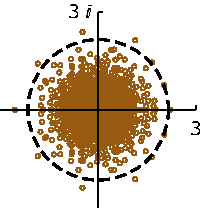
\includegraphics[width=.15\textwidth]{imgs/DOS_alpha_120_inset.pdf}}
				\put (60,-50) {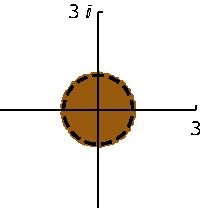
\includegraphics[width=.15\textwidth]{imgs/DOS_alpha_200_inset.pdf}}
			\end{overpic}\\
			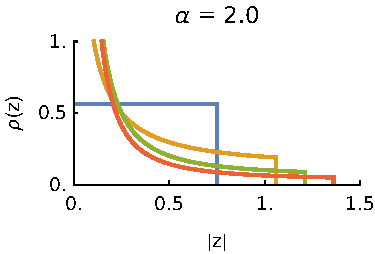
\includegraphics[width=.3\textwidth]{imgs/DOS_alpha_200.pdf}
		\end{tabular} &
		\begin{overpic}[width=.49\textwidth]{imgs/phasetransition_schematic.pdf}
			\put (0,85) {\large\textbf{(b)}}
		\end{overpic}
	\end{tabular}
	\caption{\label{fig:phase_transition}
		\textbf{Spectral density and phase diagram of heavy-tailed neural networks.} (a) Layerwise Jacobian eigenvalue density $\rho(z)$ for heavy-tailed ($\alpha = 1.2$) versus Gaussian ($\alpha = 2.0$) networks under varying weight scale parameters $D_w^{1/\alpha}$, with insets displaying empirical eigenvalue distributions and the characteristic spectral radius. (b) Phase diagram in $(\alpha, D_w^{1/\alpha})$ parameter space for $\phi = \tanh$. The fragile Gaussian edge-of-chaos critical point ($\alpha = 2.0, D_w = 1.0$) expands into a broad, two-dimensional extended critical regime for $\alpha < 2.0$, sustaining deep signal propagation without delicate parameter fine-tuning. Adapted from Qu et al. (2022).
	}
\end{figure}

Because the spectral radius alone does not capture the distribution of interior states, the capacity of the deep network to propagate signals is quantified by averaging over the Jacobian eigenvalue density:
\begin{equation}
	\mathcal{J}_f = \langle f(|\lambda_i|) \rangle = \int_{\mathbb{C}} f(|z|) \rho(z) \, dz
\end{equation}
where $f(|z|)$ is a monotonically increasing test function that penalises near-zero eigenvalues and rewards larger moduli capable of sustaining gradients across depth $L$. In Gaussian networks ($\alpha = 2$), this average is strictly maximised at the isolated critical point $D_w = 1$. 

In heavy-tailed networks ($\alpha < 2$), evaluating the ratio of Jacobian averages across the $(\alpha, D_w^{1/\alpha})$ parameter space uncovers an extended critical regime of non-zero area (Figure~\ref{fig:phase_transition}b). Within this continuous two-dimensional phase, the proportion of eigenvalues residing away from zero remains elevated, enabling learning signals and forward representations to propagate through deep architectures without requiring parameter fine-tuning. This transforms the fragile, zero-measure edge of chaos into a structurally robust critical phase.

\subsection{Anderson Multifractality and Representation Geometry}
Beyond the distribution of eigenvalue moduli, the spatial profile of the Jacobian eigenvectors governs how activity fluctuations and learned features are distributed across the network. In classical random networks with Gaussian connectivity ($\alpha = 2$), standard random matrix theory dictates that the eigenvectors of the layerwise Jacobian are delocalised. Under delocalisation, eigenvector entry magnitudes are distributed uniformly across all $N$ neurons, meaning that dynamical perturbations engage the entire system without spatial preference. 

In heavy-tailed networks ($\alpha < 2$), the spatial organisation of the Jacobian eigenstates changes, exhibiting properties characteristic of Anderson transitions in disordered physical media. To quantify the spatial localisation of a normalised Jacobian eigenmode $\mathbf{v}$, we evaluate the Inverse Participation Ratio (IPR) across a continuous moment index $q > 0$:
\begin{equation}
	\text{IPR}_q(\mathbf{v}) = \sum_{i=1}^N |v_i|^{2q} \sim N^{(1-q)D_q}
\end{equation}
where $D_q$ denotes the generalised fractal dimension. While localised states collapse to $D_q = 0$ and delocalised Gaussian states maintain $D_q \approx 1$ across all $q$, heavy-tailed networks produce spatially multifractal modes where $D_q$ is a continuous, decreasing function of $q$. These multifractal eigenvectors combine sharp, localised peaks on a sparse subset of neurons with a diffuse, delocalised background across the remaining nodes, allowing the network to operate across multiple spatial scales simultaneously.

This multifractal structure induces directional symmetry breaking in the propagation of neural representations. Because Gaussian networks possess isotropic, delocalised eigenstates, they treat all directions in activation space symmetrically; parameter configurations can only compress or nonlinearly expand representations uniformly across the entire state space. In contrast, the emergence of multifractality in the extended critical regime enables the network to simultaneously balance the expansion of task-relevant feature directions with the contraction of uninformative noise dimensions. When geometrical manifolds propagate through deep layers, this dynamic preserves input signals by concentrating the majority of activation variance into a small number of leading principal components rather than dispersing energy across the entire dimension of the layer.

The resulting representation geometry exhibits a low effective rank: internal activations populate a compact, low-dimensional subspace embedded within the wider ambient neuron space. This physical property provides a direct mechanism to address the capacity limits of continual learning systems. As established in Section 1.1, standard continual learning methods struggle to balance long-term retention with future adaptability. In Section 1.3, we examine Gradient Projection Memory, demonstrating how the emergence of low-rank, compressed feature spaces under heavy-tailed initialisation offers a principled strategy to prevent basis saturation and sustain plasticity across sequential task horizons.
\section{Gradient Projection Memory (GPM)}
To evaluate how heavy-tailed weight distributions influence continual learning, we require an algorithmic framework that isolates the geometric properties of the network without introducing confounding variables. Standard continual learning approaches often obscure these dynamics, relying on external mechanisms or heuristics that distort the optimisation trajectory. In contrast, Gradient Projection Memory (GPM), introduced by Saha et al. (2021), operates strictly via geometric subspace projections within a fixed network capacity. Because GPM relies directly on intermediate representation rank and subspace allocation, it provides a clean, deterministic baseline to evaluate how heavy-tailed initialisation alters feature compression, memory retention, and capacity usage.

\subsection{Representation-Gradient Duality}
The main mechanism of GPM relies on the geometric relationship between intermediate activations and gradient updates during backpropagation. For a fully connected layer $l$ parameterised by a weight matrix $\mathbf{W}^l \in \mathbb{R}^{d_l \times d_{l-1}}$, consider an input sample $\mathbf{x}^{l-1} \in \mathbb{R}^{d_{l-1}}$ producing pre-activation $\mathbf{h}^l = \mathbf{W}^l \mathbf{x}^{l-1} + \mathbf{b}^l$ and an incoming error vector $\boldsymbol{\delta}^l = \frac{\partial \mathcal{L}}{\partial \mathbf{h}^l} \in \mathbb{R}^{d_l}$. Applying the chain rule, the gradient of the loss $\mathcal{L}$ with respect to the weight matrix is given by the outer product:
\begin{equation}
	\nabla_{\mathbf{W}^l} \mathcal{L} = \boldsymbol{\delta}^l (\mathbf{x}^{l-1})^T \in \mathbb{R}^{d_l \times d_{l-1}}
\end{equation}
Equation (1.11) demonstrates that each row of the weight gradient matrix $\nabla_{\mathbf{W}^l} \mathcal{L}$ lies strictly within the vector space spanned by the incoming post-activation representation $\mathbf{x}^{l-1}$. This creates an intrinsic duality between activations and parameter updates: the subspace spanned by a task's feature representations directly defines the subspace where gradient steps modify the layer's connections. 

Leveraging this relationship, GPM divides the gradient space of each layer into two mutually orthogonal subspaces:
The Core Gradient Space (CGS) represents the subspace spanned by the dominant feature representations of past tasks. Taking parameter updates within this subspace alters historical representations, overwriting past knowledge and triggering catastrophic forgetting. Conversely, the Residual Gradient Space (RGS) constitutes the orthogonal complement of the Core Gradient Space. Gradient steps executed within the Residual Gradient Space act orthogonally to past activation vectors, leaving past feature mappings intact while freeing the remaining parametric degrees of freedom to learn novel tasks.

\begin{figure}[htbp]
	\centering
	\vspace*{-2em}
	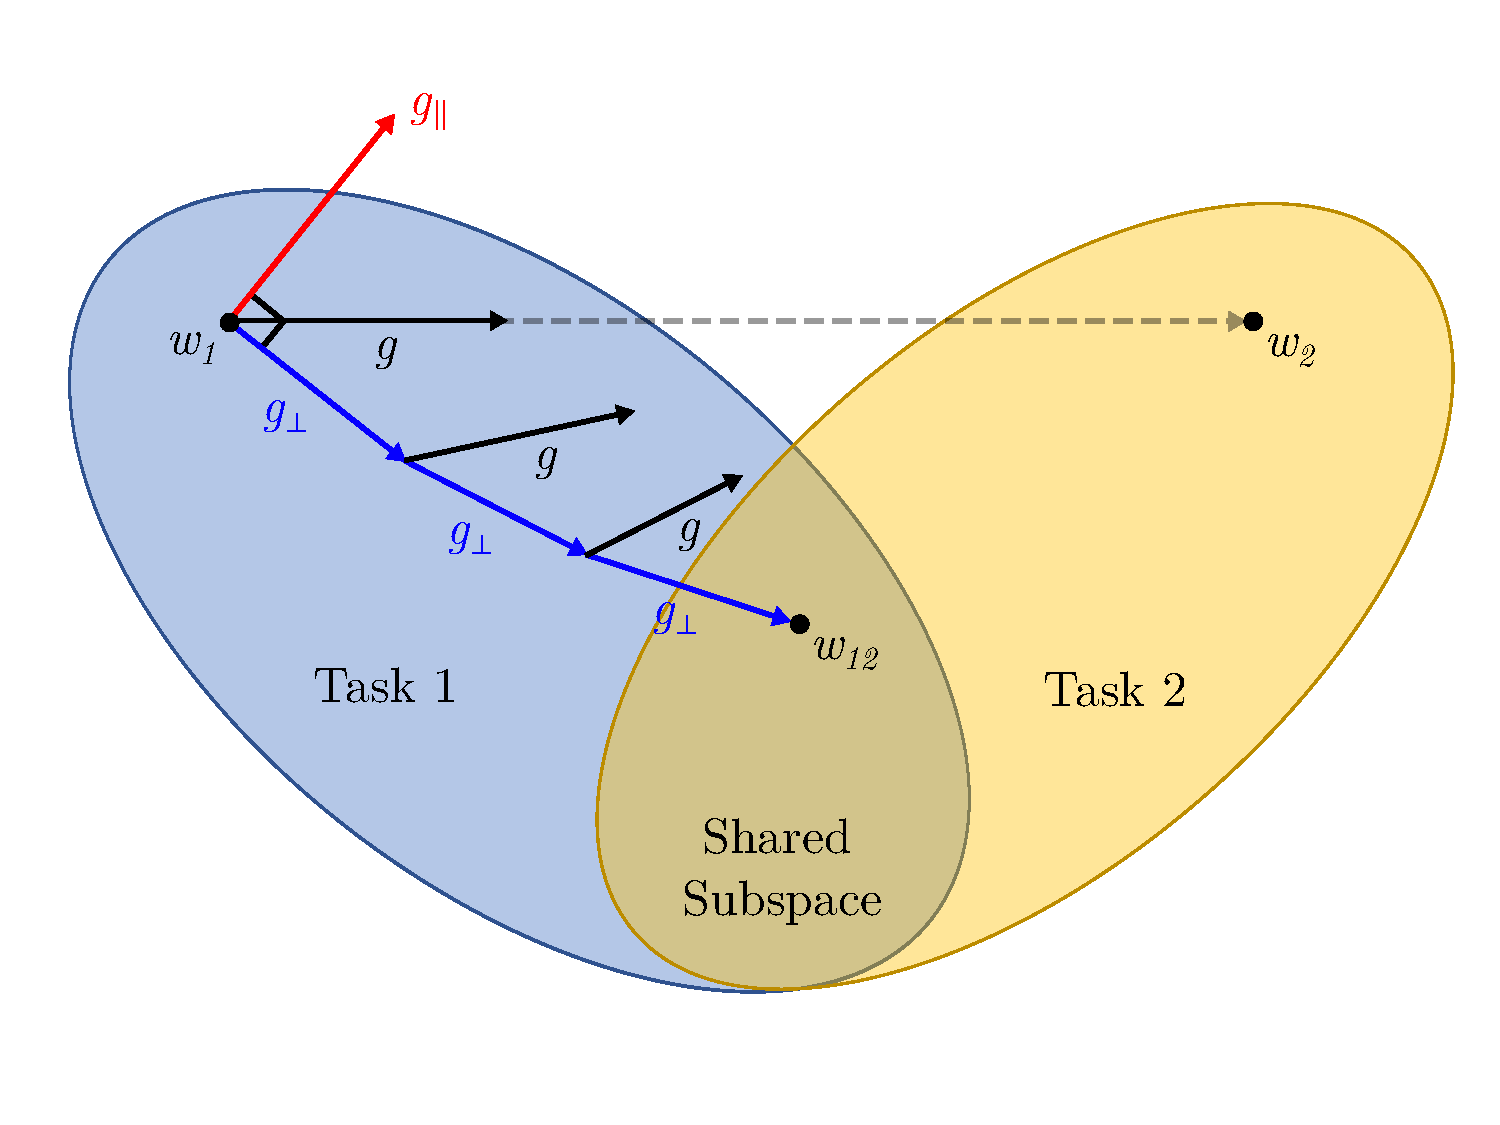
\includegraphics[width=0.7\textwidth]{imgs/gpm.pdf}
	\vspace*{-2em}
	\caption{\textbf{Geometric mechanism of Gradient Projection Memory across sequential tasks.} After optimising Task 1 to parameter configuration $w_1$, standard optimisation computes gradient updates $g$ driven purely by Task 2 (dashed trajectory), which steer parameters toward $w_2$ and cause catastrophic forgetting by leaving the Task 1 subspace. GPM decomposes $g$ into an interfering parallel component $g_\parallel$ aligned with past representation directions and an orthogonal projection $g_\perp$ residing in the residual gradient space. Updating parameters strictly along $g_\perp$ guides the trajectory along the boundary of Task 1 into a joint configuration $w_{12}$ within the shared subspace, allowing the network to acquire Task 2 while preserving past task performance.}
	\label{fig:gpm}
\end{figure}

\subsection{Basis Construction and Projection Dynamics}
To isolate the Core Gradient Space upon completing Task 1, GPM collects post-activation vectors from a calibration set of $n_s$ samples into a representation matrix $\mathbf{R}_1^l \in \mathbb{R}^{d_{l-1} \times n_s}$ for each layer $l$. Applying Singular Value Decomposition (SVD), $\mathbf{R}_1^l = \mathbf{U}_1^l \mathbf{\Sigma}_1^l (\mathbf{V}_1^l)^T$, extracts an orthonormal basis spanning the activation space. The top $k_1$ left singular vectors that capture the majority of activation variance are retained according to an energy threshold $\epsilon_{\text{th}}^l \in (0, 1]$:
\begin{equation}
	\left\| (\mathbf{R}_1^l)_{k_1} \right\|_F^2 \ge \epsilon_{\text{th}}^l \left\| \mathbf{R}_1^l \right\|_F^2
\end{equation}
where $\|\cdot\|_F$ denotes the Frobenius norm. Storing these vectors yields the initial basis matrix $\mathbf{M}^l = [\mathbf{u}_{1,1}^l, \dots, \mathbf{u}_{k_1,1}^l] \in \mathbb{R}^{d_{l-1} \times k_1}$ defining the protected subspace for Task 1.

When training subsequent tasks ($t \ge 2$), incoming backpropagated gradients $\nabla_{\mathbf{W}_t^l} \mathcal{L}_t$ are constrained by projecting them onto the orthogonal complement of the stored memory before updating weights:
\begin{equation}
	\nabla_{\mathbf{W}_t^l} \mathcal{L}_t^{\text{proj}} = \nabla_{\mathbf{W}_t^l} \mathcal{L}_t \left( \mathbf{I} - \mathbf{M}^l (\mathbf{M}^l)^T \right)
\end{equation}
Because $(\mathbf{M}^l)^T \nabla_{\mathbf{W}_t^l} \mathcal{L}_t^{\text{proj}} = \mathbf{0}$, weight updates satisfy $\Delta \mathbf{W}_t^l \mathbf{x}_{<t}^{l-1} \approx \mathbf{0}$, preserving historical mappings without altering the objective function. Upon completing task $t$, new representations are incorporated without redundancy by projecting the current activation matrix $\mathbf{R}_t^l$ onto the residual subspace: $\hat{\mathbf{R}}_t^l = (\mathbf{I} - \mathbf{M}^l (\mathbf{M}^l)^T) \mathbf{R}_t^l$. Applying SVD to $\hat{\mathbf{R}}_t^l$ yields $k_{\text{new}}$ newly identified singular vectors meeting the threshold $\epsilon_{\text{th}}^l$, which are appended to expand the orthonormal basis: $\mathbf{M}^l \leftarrow [\mathbf{M}^l, \, \hat{\mathbf{u}}_{1,t}^l, \dots, \hat{\mathbf{u}}_{k_{\text{new}},t}^l]$.
\subsection{Subspace Saturation and Effective Rank}
Because layer dimensions are finite, appending $k_j$ orthogonal basis vectors after each task monotonically contracts the Residual Gradient Space:
\begin{equation}
	\dim(\text{RGS}^l) = d_{l-1} - K_t
\end{equation}
where $K_t = \sum_{j=1}^t k_j$ is the cumulative basis count across $t$ completed tasks. The contraction rate depends directly on the spectral decay of intermediate activations. When representations exhibit high effective rank, dispersing variance across many singular modes, satisfying the energy threshold $\epsilon_{\text{th}}^l$ requires storing large basis sets $k_j$ per task, causing $K_t$ to rapidly approach the ambient layer dimension $d_{l-1}$.

When the accumulated memory spans the full representation space ($K_t = d_{l-1}$), the projection operator collapses to zero ($\mathbf{I} - \mathbf{M}^l (\mathbf{M}^l)^T = \mathbf{0}$), projecting all incoming gradients to zero ($\nabla_{\mathbf{W}_t^l} \mathcal{L}_t^{\text{proj}} = \mathbf{0}$) and inducing an irreversible loss of plasticity. Adjusting the energy threshold $\epsilon_{\text{th}}^l$ merely trades catastrophic forgetting for accelerated saturation without resolving this dimensional ceiling. Consequently, GPM's operational lifespan is bounded by representation rank. This limitation motivates our investigation into heavy-tailed initialisation: by inducing directional symmetry breaking and compressing feature rank at step zero, heavy-tailed networks slow basis accumulation and preserve residual gradient capacity across extended task sequences.
\chapter{Representational Geometry}
\label{chap:chap2}

\chapter{Continual Learning Dynamics}
\label{chap:chap3}

\chapter{Extension to Modern Architectures}
\label{chap:chap4}

\chapter{Discussion}
\label{chap:chap5}

% ---------------------------------------------------------
% REFERENCES
% ---------------------------------------------------------
% Only the first page counts toward the 40-page limit.
\newpage
\addcontentsline{toc}{chapter}{References}
\nocite{*}
\printbibliography[heading=bibintoc, title={References}]

% ---------------------------------------------------------
% APPENDICES
% ---------------------------------------------------------
% Not part of the 40-page limit.
\appendix
\chapter{Computer Code}
Relevant snippets of the PyTorch implementation and the Lévy-stable initialisation logic are included here. The full repository can be found at: \url{https://github.com/YiHaoFromEarth/ht-initialisation-dynamics}

\end{document}
